\documentclass[12pt]{article} % Định dạng tài liệu kích thước chữ 12pt

\usepackage{polyglossia} % Quản lí ngôn ngữ
\setdefaultlanguage{vietnamese}
\setotherlanguages{english}
\usepackage{fontspec} % Cung cấp khả năng sử dụng ngôn phông chữ OpenType và TrueType
\usepackage{
    amsmath, % Các lệnh toán học
    amsfonts, % Các kí hiệu toán học
    amssymb % Các kí hiệu toán học
}
\usepackage{unicode-math} % Cung cấp hỗ trợ cho các phông chữ toán học Unicode
\setmainfont{STIX Two Text} % Thiết lập phông chữ chính là STIX Two Text
\setmathfont{STIX Two Math} % Thiết lập phông chữ toán học là STIX Two Math

% \setmainfont{Noto Serif} % Đậm nhưng chữ hơi to
% \setmathfont{Noto Serif}
% \setmainfont{DejaVu Serif}
% \setmathfont{DejaVu Serif}
% \setmainfont{Libertinus Serif}
% \setmathfont{Libertinus Math}
% \setmainfont{TeX Gyre Pagella}
% \setmathfont{TeX Gyre Pagella Math}
% \setmainfont{Latin Modern Roman}
% \setmathfont{Latin Modern Math}
% \setmainfont{XITS} % Xấu nhất, lỗi dấu dính vào mũ
% \setmathfont{XITS Math}
%\setmainfont{IBM Plex Serif}
%\setmathfont{IBM Plex Math}
% \setmainfont{TeX Gyre Termes}
% \setmathfont{TeX Gyre Termes Math}

% \usepackage{enumitem} % Quản lí các danh sách (không sử dụng ở đây)
% \usepackage{cleveref} % Cung cấp các lệnh tham chiếu thông minh (không sử dụng ở đây)
%\usepackage[backend=biber,style=numeric]{biblatex} % Quản lí tài liệu tham khảo với biber và kiểu numeric

\usepackage[a4paper, left=2cm, right=2cm, top=2cm, bottom=2cm]{geometry} % Định dạng kích thước và lề trang 
\usepackage{graphicx} % Hỗ trợ chèn hình ảnh vào tài liệu
\usepackage{xcolor} % Gói màu sắc để tùy chỉnh màu sắc
\usepackage[vietnamese]{hyperref} % Tạo liên kết và tham chiếu trong tài liệu, hỗ trợ tiếng Việt
\usepackage{bookmark} % Tạo mục lục nhanh và chính xác hơn
% \usepackage{cleveref} % Cung cấp các lệnh tham chiếu thông minh (không sử dụng ở đây)
\hypersetup{
    colorlinks=true, % Kích hoạt màu sắc cho các liên kết
    linkcolor=darkgray,    % Màu của liên kết nội bộ
    citecolor=blue,    % Màu của liên kết tham chiếu
    filecolor=blue,    % Màu của liên kết tập tin
    urlcolor=blue      % Màu của liên kết URL
}
\renewcommand{\sectionautorefname}{Mục} % Đổi tên tự động của các liến kết phần mục từ "Section" thành "Mục"

% Quản lí tài liệu tham khảo
\usepackage[backend=biber,style=numeric]{biblatex} % Quản lí tài liệu tham khảo với biber và kiểu numeric
\addbibresource{references.bib} % Thêm tài liệu tham khảo từ tệp references.bib
\DeclareLanguageMapping{vietnamese}{vietnamese-english} % Định nghĩa ánh xạ ngôn ngữ cho tiếng Việt
\DeclareLanguageMapping{english}{english} % Định nghĩa ánh xạ ngôn ngữ cho tiếng anh

% Định nghĩa môi trường Bài Tập
\newcounter{baitap} % Tạo một bộ đếm mới cho bài tập
\newenvironment{baitap}[1][]{%
    \noindent\textsc{Bài tập #1}\par % Định dạng tiêu đề môi trường bài tập
    \noindent
}{%
    \par
}
\newenvironment{baitap1}[1][]{%
    \refstepcounter{baitap}% Tăng số đếm của môi trường bài tập 
    \noindent\textsc{Bài tập \thebaitap #1}\par % Định dạng tiêu đề môi trường bài tập với số đếm
    \noindent
}{%
    \par
}

\title{Khai triển lũy thừa \texorpdfstring{\((1+x)^n\)}{nhị thức} thành đa thức} % Tiêu đề tài liệu có công thức toán học
\author{Nguyễn Tấn Nhựt}
\date{\today}

\allowdisplaybreaks % Cho phép gãy dòng trong các công thức toán học dài

%===============================================

\begin{document}

\maketitle

%%%%%%%%%%

\section{Dẫn nhập} \label{sec:dan-nhap}
Khai triển biểu thức là biến đổi biểu thức từ dạng này sang dạng khác, thường là từ dạng phức tạp sang dạng đơn giản, hoặc từ một dạng trừu tượng sang dạng chứa các thành phần cụ thể. Mục tiêu của việc này là làm cho biểu thức trở nên dễ hiểu hơn và dễ thao tác hơn trong các phép toán. Vấn đề đang xét là khai triển biểu thức \((1+x)^n\) thành đa thức. Ví dụ, \((1+x)^2\) được khai triển thành \(1+2x+x^2\). 

Biểu thức \((1+x)^2\) là một trường hợp riêng của biểu thức \((x+y)^2\) khi \(y=1\), nhưng khi biết dạng khai triển của cái trước vẫn có thể suy ra dạng khai triển của cái sau. Để thấy điều này, với \(x\ne 0\), hãy quan sát 
    \begin{align*}
        (x+y)^2
            &=x^2\left(1+\frac{y}{x}\right)^2 \\
            &=x^2\left[1+2\left(\frac{y}{x}\right)+\left(\frac{y}{x}\right)^2\right] \\
            &=x^2+2xy+y^2.
    \end{align*}
Tương tự như vậy, việc nghiên cứu dạng khai triển của \((1+x)^n\) không làm mất tính tổng quát của bài toán, vì cũng có
\[(x+y)^n=x^n\left(1+\frac{y}{x}\right)^n.\]

Để ngắn gọn và đạt hiệu quả truyền đạt cao hơn trong khi lập luận, gọi \(s_n\) là dạng khai triển của \((1+x)^n\). Ví dụ, \(s_2\) là \(1+2x+x^2\). Khi nói đến \(s_2\), hãy nghĩ đến \(1+2x+x^2\), đừng nghĩ đến \((1+x)^2\) hay các dạng trung gian. Để hoàn thiện bài toán, chúng ta cũng cần xác định hai trường hợp đặc biệt, \((1+x)^0=1\) theo qui ước và \((1+x)^1=1+x\) là tầm thường. Kể từ đây, \(n\) được hiểu là một số nguyên không âm, \(s_0=1\) và \(s_1=1+x\).

Vì biểu thức \(1+x\) hay \(x+y\) có dạng nhị thức, chúng ta gọi việc khai triển biểu thức \((1+x)^n\) hay \((x+y)^n\) là \emph{khai triển nhị thức}. Mục tiêu của chúng ta là xác định \(s_n\) và kết quả này được gọi là \emph{định lí nhị thức}.

%%%%%%%%%%%
\section{Tiếp cận trực tiếp}
Cách trực tiếp nghiên cứu dáng điệu \(s_n\) là nhân phân phối. Tôi sẽ bắt đầu với một số trường hợp đơn giản như 
\begin{align*}
    (1+x)^2
        & = (1+x)(1+x) \\
        & = (1+x)1 + (1+x)x \\
        & = 1 \cdot 1 + x \cdot 1 + 1 \cdot x + x \cdot x \\
        & = 1 + x + x +x^2 \\
        & = 1 + 2x + x^2, \\
    (1+x)^3 
        & = (1+x)^2(1+x) \\
        & = (1 \cdot 1 + x \cdot 1 + 1 \cdot x + x \cdot x)(1+x) \\
        & = (1 \cdot 1 + x \cdot 1 + 1 \cdot x + x \cdot x) 1 + (1 \cdot 1 + x \cdot 1 + 1 \cdot x + x \cdot x) x \\
        & = 1 \cdot 1 \cdot 1 + x \cdot 1 \cdot 1 + 1 \cdot x \cdot 1 + x \cdot x \cdot 1 \\
        & \quad + 1 \cdot 1 \cdot x + x \cdot 1 \cdot x + 1 \cdot x \cdot x + x \cdot x \cdot x \\
        & = 1 + x + x + x^2 + x + x^2 + x^2 + x^3 \\
        & = 1 + 3x + 3x^2 + x^3.
\end{align*}
Hãy quan sát và ghi nhận những điều sau đây.
\begin{itemize}
    \item Nhân 2 nhị thức với nhau, tổng thu được có 4 hạng tử, mỗi hạng tử có 2 nhân tử. Các hạng tử được thu gọn sẽ có một trong các dạng \(1, x, x^2\). Tổng được thu gọn sẽ còn lại 3 hạng tử, \(1+2x+x^2\), đây chính là \(s_2\).        
    \item Nhân 3 nhị thức với nhau, tổng thu được có 8 hạng tử, mỗi hạng tử có 3 nhân tử, mỗi hạng tử có 3 nhân tử. Các hạng tử được thu gọn sẽ có một trong các dạng \(1, x, x^2, x^3\). Tổng được thu gọn sẽ còn lại 4 hạng tử, \(1+3x+3x^2+x^3\), đây chính là \(s_3\).
\end{itemize} 

Trường hợp tổng quát, tích \((1+x)(1+x)\cdots(1+x)\). Việc đó được thực hiện bằng cách, đầu tiên, từ mỗi nhị thức, lấy ra một hạng tử, hoặc là \(1\) hoặc là \(x\), lập chúng thành một tích, mà trong tích này hạng tử lấy ra từ nhị thức nào sẽ đứng đúng vị trí nhị thức đó như trong tích các nhị thức. Sau đó, lấy tổng tất cả các tích này, nó chính là tích của \(n\) nhị thức ban đầu. Dưới đây là công thức hình thức biểu diễn tổng này, 
\[
(1+x)_1(1+x)_2\cdots(1+x)_n
    = \sum_{\substack{b_1 \text{ hoặc là } 1 \text{ hoặc là } x \text{ từ } (1+x)_1 \\ b_2 \text{ hoặc là } 1 \text{ hoặc là } x \text{ từ } (1+x)_2 \\ \vdots \\ b_n \text{ hoặc là } 1 \text{ hoặc là } x \text{ từ } (1+x)_n  }} b_1 b_2 \cdots b_n.
\]
% Hãy giải thích công thức này, mặc dù sau đó hãy quên nó đi, nó không có tác dụng gì đặc biệt về sau, tuy nhiên tại sao tôi đưa nó ra ở đây và tại sao bạn cần biết nó, bạn có thể tự rút ra bài học cho mình hay không, đó là tùy vào bạn, riêng tôi học được không ít từ nó. Thứ nhất, các chỉ số dưới chỉ ra vị trí tương ứng của các nhân tử trong tích, nó cho biết, chẳng hạn \(b_1\) là số hạng được rút ra từ nhị thức thứ nhất, tức là \((1+x)_1\). Thứ hai, tập \(\{(1,x\}^n\) chính là 
% \[
% \{(1, 1, \dots, 1); (1, 1, \dots, x);\dots; (x, x, \dots, x)\}
% \]

Điều trở ngại là tìm phương thức liệt kê hiệu quả, tức không bỏ sót và gây nhầm lẫn, tất cả các hạng tử thu được từ việc nhân \(n\) nhị thức đó với nhau.

Nhân \(n\) nhị thức với nhau, tổng thu được có \(2^n\) hạng tử, mỗi hạng tử có \(n\) nhân tử. Mỗi hạng tử có \(n\) nhân tử là hiển nhiên, nhưng vì sao lại có \(2^n\) hạng tử? Hãy hình dung mỗi hạng tử là một dãy \(n\) ô vuông, mỗi ô vuông đại diện cho một nhân tử của hạng tử. Có thể đưa vào mỗi ô vuông hoặc \(1\) hoặc \(x\) được lấy ra từ nhị thức \(1+x\). Bây giờ, liệu bạn có thể đếm được có bao nhiêu hạng tử hay không? Số hạng tử chính là số cách tạo nên một hạng tử. Để tạo nên một hạng tử, nhân tử thứ nhất của hạng tử có 2 cách chọn hoặc \(1\) hoặc \(x\), nhân tử thứ 2 cũng vậy, vân vân, cho đến nhân tử thứ \(n\) cũng vậy. Từ đó, suy ra có \(2\cdot 2\cdots 2\) hay \(2^n\) cách thành lập một hạng tử.

\begin{figure}[h!]
    \centering
    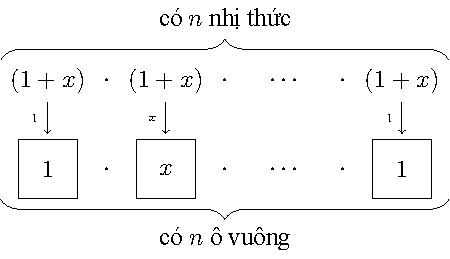
\includegraphics[scale=1]{../images/luoi_n_o_vuong/luoi_n_o_vuong.pdf}
    \caption{Minh họa cách thức hình thành một hạng tử.}
    % \label{fig:example}
\end{figure}

Khi các hạng tử được viết dưới dạng lũy thừa, các dạng của chúng là \(1, x, x^2, \dots, x^j, \dots, x^n\). Trong đó, hạng tử \(1\) là tích của \(n\) nhân tử giống nhau \(1\), 
    \[1=\underbrace{1 \cdot 1 \cdot \cdots \cdot 1}_{\text{có \(n\) nhân tử 1}},\]
và số hạng \(x^n\) là tích của \(n\) nhân tử giống nhau \(x\),
    \[x^n=\underbrace{x \cdot x \cdot \cdots \cdot x}_{\text{có \(n\) nhân tử x}}.\]
Hai số hạng này, \(1\) và \(x^n\), mỗi số hạng xuất hiện một lần. Các số hạng còn lại, mỗi số hạng đều xuất hiện nhiều lần, quan trọng là phải biết số lần xuất hiện đó. Gọi \(c(0)\) là số lần xuất hiện của \(x^0\) hay \(1\), \(c(1)\) là số lần xuất hiện \(x^1\), \(c(2)\) là số lần xuất hiện \(x^2\), cho đến \(c(n)\) là số lần xuất hiện \(x^n\). Lưu ý, \(c(0)=c(n)=1\) đã trình bày. Như vậy, có thể tạm đưa ra công thức
    \[s_n=1+c(1)x^1+c(2)x^2+\cdots+x^n\]
hay
    \[s_n=c(0)x^0+c(1)x^1+c(2)x^2+\cdots+c(n)x^n.\]
Hoặc cũng có thể viết theo dạng tổng xít-mờ là
    \[s_n=\sum_{j=0}^nc(j)x^j,\]
ở đây, \(c(j)\) là số lần xuất hiện \(x^j\), với \(j\) là một trong các số từ \(0\) đến \(n\). 

Nhiệm vụ bày ra là tìm \(c(j)\), cần nhấn mạnh nó chính là số lần xuất hiện hạng tử \(x^j\).

    \begin{figure}[h!]
        \centering
        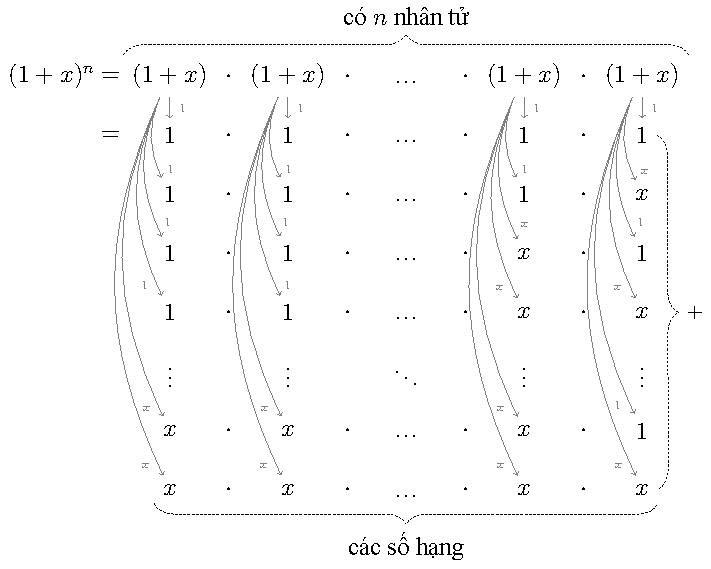
\includegraphics[scale=1]{../images/hang_tu_cau_truc/hang_tu_cau_truc.pdf}
        \caption{Mô tả việc thực hiện các phép nhân để khai triển tích thành tổng các hạng tử.}
        % \label{fig:example}
    \end{figure}
Dưới đây là các bước liệt kê tất các hạng tử khi thực hiện phép nhân mà không sợ bỏ sót.
    \begin{itemize}
        \item [Bước 1] Hạng tử thứ nhất là 
            \[1 \cdot 1 \cdots 1 \cdots 1 \cdot 1 \cdot 1.\] 
        \item [Bước 2] Hạng tử thứ hai là 
            \[1 \cdot 1 \cdots 1 \cdots 1 \cdot 1 \cdot x.\] 
        Đây là hạng tử thứ nhất mà nhân tử thứ \(n\) từ \(1\) đã được thay thế bởi \(x\).
        \item [Bước 3] Hạng tử thứ ba và thứ tư là 
            \[\begin{matrix}
                1 \cdot 1 \cdots 1 \cdots 1 \cdot x \cdot 1, \\
                1 \cdot 1 \cdots 1 \cdots 1 \cdot x \cdot x.
            \end{matrix}\]
        Hạng tử thứ ba do hạng tử thứ nhất tạo thành bằng cách thay nhân tử thứ \(n-1\) từ \(1\) bởi \(x\). Hạng tử thứ tư do hạng tử thứ hai tạo thành bằng cách thay nhân tử thứ \(n-1\) từ \(1\) bởi \(x\). 
        \item [Bước 4] Các hạng tử từ thứ năm đến thứ tám là
            \[\begin{matrix}
                1 \cdot 1 \cdots 1 \cdots x \cdot 1 \cdot 1, \\
                1 \cdot 1 \cdots 1 \cdots x \cdot 1 \cdot x, \\
                1 \cdot 1 \cdots 1 \cdots x \cdot x \cdot 1, \\
                1 \cdot 1 \cdots 1 \cdots x \cdot x \cdot x.
            \end{matrix}\]
        \item [Bước \(n\)] Có thêm \(2^{n-2}\) hạng tử, có tổng cộng \(2^{n-1}\) hạng tử.
            \[\begin{matrix}
                1 \cdot x \cdots 1 \cdots 1 \cdot 1 \cdot 1, \\
                1 \cdot x \cdots 1 \cdots 1 \cdot 1 \cdot x, \\
                1 \cdot x \cdots 1 \cdots 1 \cdot x \cdot 1, \\
                1 \cdot x \cdots 1 \cdots 1 \cdot x \cdot x, \\
                1 \cdot x \cdots 1 \cdots x \cdot 1 \cdot 1, \\
                1 \cdot x \cdots 1 \cdots x \cdot 1 \cdot x, \\
                1 \cdot x \cdots 1 \cdots x \cdot x \cdot 1, \\
                1 \cdot x \cdots 1 \cdots x \cdot x \cdot x, \\
                \dots \\
                1 \cdot x \cdots x \cdots x \cdot x \cdot x.
            \end{matrix}\]
        \item [Bước \(n+1\)] Có thêm \(2^{n-1}\) hạng tử, có tổng cộng \(2^{n}\) hạng tử.
    \end{itemize} 
    Hãy viết một chương trình máy tính bằng một ngôn ngữ lập trình phù hợp, khi nhập vào \(n\), chương trình liệt kê cho ta tất cả các hạng tử như trên.

\end{document}














Hai hạng tử \(1\) và \(x^n\) là các hạng tử duy nhất của bất kì \(s_n\) được nhìn thấy khi viết \((1+x)^n\) dưới dạng tích, đó là
\[\underbrace{(1+x)(1+x)\cdots(1+x)}_{\text{có } n \text{ thừa số}}.\]
Khi tiến hành nhân phân phối tích này, lúc nào cũng thu được
\begin{align*}
    1 & = \underbrace{1 \cdot 1 \cdot \cdots \cdot 1}_{\text{có } n \text{ nhân tử}} \\
    \noalign{\noindent\hspace{0pt}\text{và}} \\
    x^n & = \underbrace{x \cdot x \cdot \cdots \cdot x}_{\text{có } n \text{ nhân tử}}.
\end{align*}

Quan sát tháp trong \autoref{fig:thap-tim-s5}, thấy rằng hệ số của \(x^j\) ở hàng dưới là tổng của hệ số của \(x^{j-1}\) và \(x^j\) ở hàng liền trên, \(1\leq j \leq 5\) . Ví dụ, hệ số của \(x^4\) ở hàng thứ sáu là tổng của hệ số của \(x^3\) và \(x^4\) ở hàng thứ năm, \(5=4+1\). Bên cạnh đó, trong cùng một hàng, hệ số của \(x^{j}\) bằng với hệ số của \(x^{n-j}\). Ví dụ, ở hàng thứ sáu, hệ số của \(x\) và \(x^4\) cùng bằng \(5\).

Y cứ trên những điểm quan sát được từ \autoref{fig:thap-tim-s5}, đề xuất giả thiết qui nạp 
\begin{align}
    s_{n-1}&=\binom{n-1}{0}+\binom{n-1}{1}x+\cdots+\binom{n-1}{n-2}x^{n-2}+\binom{n-1}{n-1}x^{n-1}\tag*{}\\
    s_n&=\binom{n}{0}+\binom{n}{1}x+\cdots+\binom{n}{n-1}x^{n-1}+\binom{n}{n}x^n \label{eq:dang-khai-trien}
\end{align}
mà trong đó, 
\begin{align}
    \binom{n}{j}=\binom{n-1}{j-1}+\binom{n-1}{j} \label{eq:tinh-he-so-nhi-thuc-theo-chieu-doc}
\end{align}
đúng với mọi \(j\) sao cho \(1\leq j\leq n\), và
\begin{align}
    \binom{n}{j}=\binom{n}{n-j} \label{eq:tinh-doi-xung}
\end{align}
đúng với mọi \(j\) sao cho \(0\leq j\leq n\).